\newcommand{\balance}{\prg{bal}}
\newcommand{\password}{\prg{pwd}}
\newcommand{\myAccount}{\prg{accnt}}

\section{Questions arising from "deeper" mofifications of the heap}

 So far, we have considered pretty "flat" examples, where consider  at most one field read. Consider now a module with \prg{Account}s and\prg{Shop}s as below

\begin{lstlisting}[mathescape=true, language=Chainmail, frame=lines]
module $M_{as}$        
  class Password
  
  class Account
    ... as in $\ModC$
    
   class Shop
       field acc: Account
       
       method swap(a:Account)
          this.acc = a
    
\end{lstlisting}
%
  
We use the notation ${\inside{x}}$ to say that $x$ is protected. Assume that we want $M_{as}$   to satisfy

 \begin{tabular}{lcll}
 $S_{as}$   & $\triangleq$   &  $\TwoStatesQ {\prg{s}:\prg{Shop}}  {\inside{\prg{s.acc.pwd}}}  {\inside{\prg{s.acc.pwd}}}$
 \end{tabular}
  
\subsection{Changing footprints}  

Note that the ``footprint'' of $S_{as}$ in the pre-state may be different than that on the post-state. For example, if we have a shop a in the original configuration below,  and execute \prg{s.swap(4)}. then we obtain the configuration to the right. In the original configuration the footprint of \prg{5.acc.pwd} consists of $\{ 1. 2, 3\}$, but in the second configuration it consists of $\{ 1. 4, 5\}$
  
\begin{figure}[htb]
\begin{tabular}{|c|c|}
\hline \\
\resizebox{4.5cm}{!}{
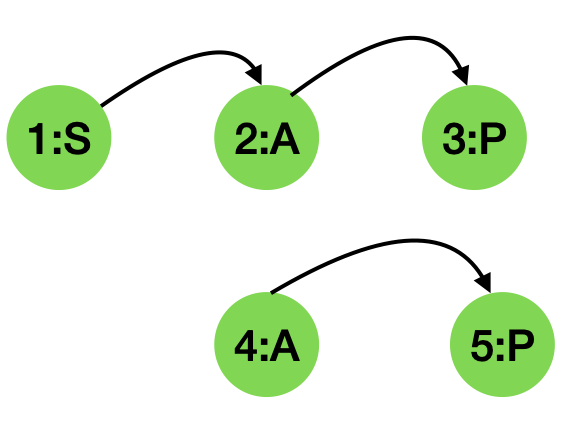
\includegraphics[width=\linewidth]{diagrams/scenarioOne.png}
} 
&
\resizebox{4.5cm}{!}{
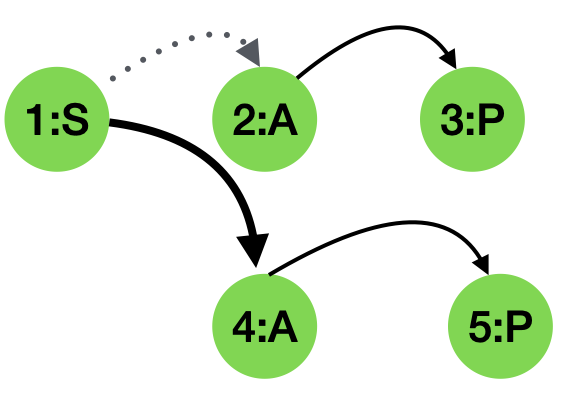
\includegraphics[width=\linewidth]{diagrams/scenarioTwo.png}
} 
\\
\hline
original configuration
&
 configuration after executing \prg{1.swap(4)}
\\
\hline \hline
\end{tabular}
   \caption{changing footprint}
   \label{fig:ScenarioA}
 \end{figure}
 
\subsection{Proving method \prg{swap}}

We can give yo  \prg{Swap}  he following pre- and post- condition pair


\subsection{First Worry}

\begin{figure}[htb]
\begin{tabular}{|c|c|cl}
\hline \\
\resizebox{4.1cm}{!}{
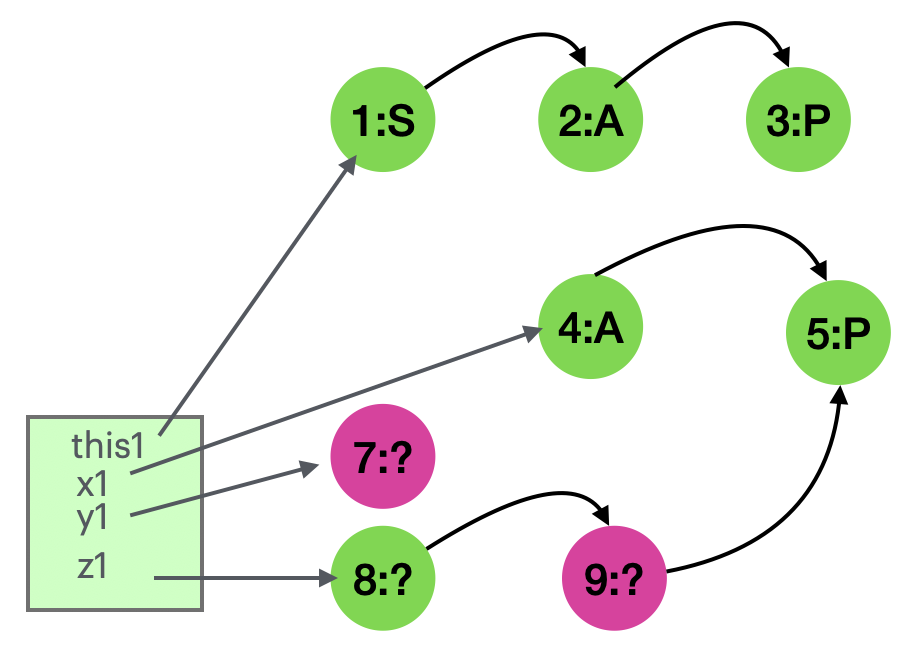
\includegraphics[width=\linewidth]{diagrams/scenarioBOne.png}
} 
&
\resizebox{4.1cm}{!}{
\includegraphics[width=\linewidth]{diagrams/scenarioBTwo.png}
} 
&
\resizebox{4.1cm}{!}{
\includegraphics[width=\linewidth]{diagrams/scenarioBThree.png}
} 
\\
\hline
$\sigma_1$
&
$\sigma_2$
&
$\sigma_3$
\\
\small{$..,\sigma_1 \models {\protectedFrom {\prg{this.acc.pwd}} {\{ \prg{x}, \prg{y}, \prg{z} \}} }$}
&
$..,\sigma_2 \models {\inside {\prg{x.acc.pwd}}}$
&
$..,\sigma_3 \models {\inside {\prg{this.acc.pwd}}} $
\\
\small{$..,\sigma_1 \not\models {\protectedFrom {\prg{x.pwd}} { \prg{z}  }}$} & & 
\\
\hline \hline
\resizebox{4.1cm}{!}{
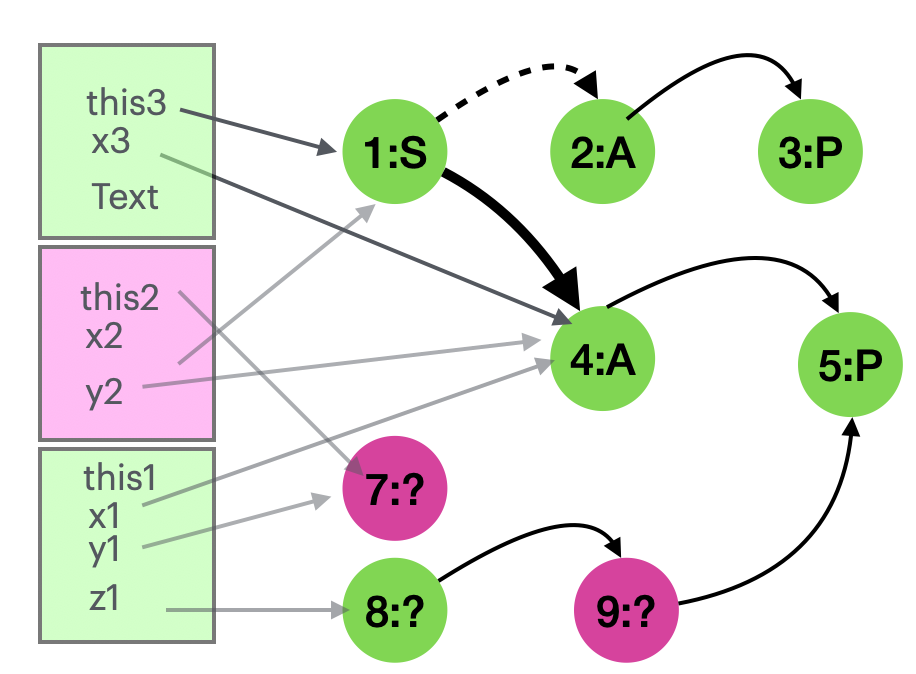
\includegraphics[width=\linewidth]{diagrams/scenarioBFour.png}
} 
&
\resizebox{4.1cm}{!}{
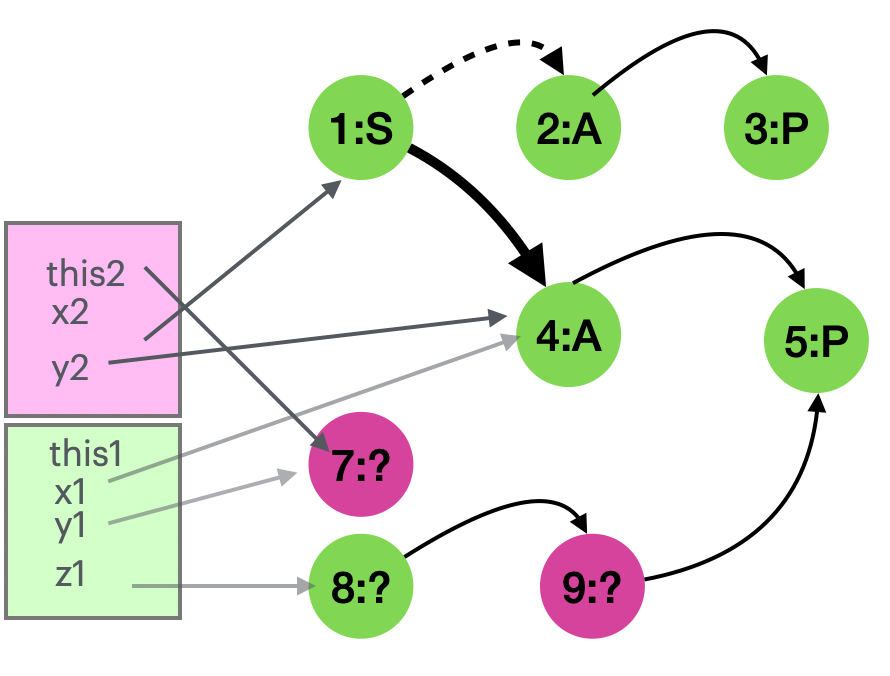
\includegraphics[width=\linewidth]{diagrams/scenarioBFive.png}
}
&
\resizebox{4.1cm}{!}{
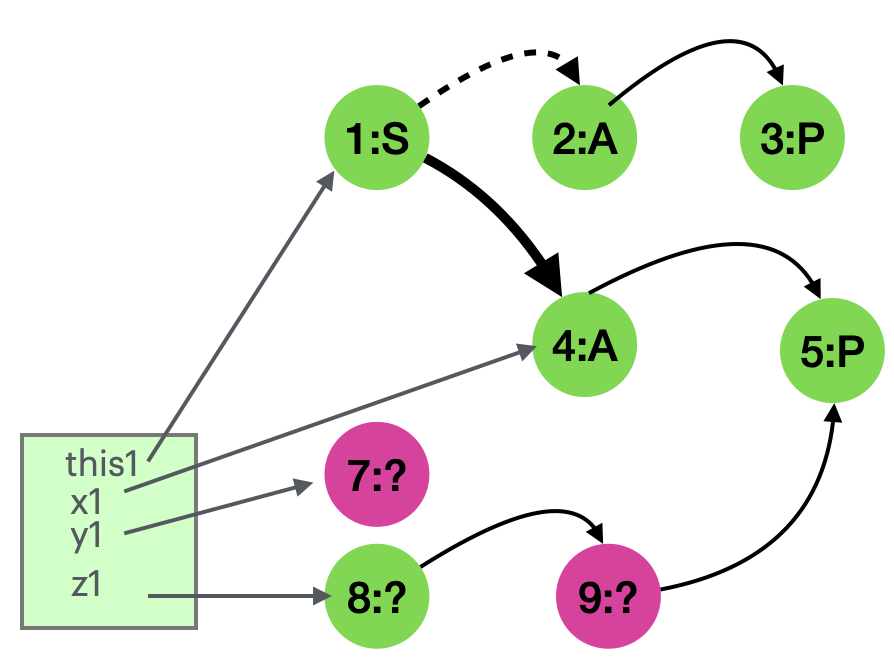
\includegraphics[width=\linewidth]{diagrams/scenarioBSix.png}
} 
\\
\hline 
$\sigma_4$
&
$\sigma_5$
&
$\sigma_6$
\\
$..,\sigma_4 \models {\inside {\prg{this.acc.pwd}}}$
&
$..,\sigma_5 \models {\inside {\prg{x.acc.pwd}}}$
&
\small{$..,\sigma_6 \not\models {\protectedFrom {\prg{this.acc.pwd}} {\{ \prg{x}, \prg{y}, \prg{z} \}} }$}
\\
\hline 
\hline
\end{tabular}
   \caption{calling \prg{swap} and exposing the password?}
   \label{fig:ScenarioB}
 \end{figure}


 
 
